% add "showtrims" to class options to show the trimming lines
% add draft for preview without images
\documentclass[10pt,twoside,openany,x11names,svgnames,italian,a4paper,dvipsnames,table]{memoir}
\usepackage{amssymb}
\usepackage[italian]{babel}
\usepackage[T1]{fontenc}
\usepackage{wrapfig}
\usepackage{tikz}
\newcommand{\tikzcircle}[2][red,fill=red]{\tikz[baseline=-0.5ex]\draw[#1,radius=#2] (0,0) circle ;}%
\usepackage{ifxetex}
\usepackage{ragged2e}

\setstocksize{303mm}{215mm}
\settrimmedsize{297mm}{210mm}{*}
\settrims{3mm}{3mm}

% Apply and enforce layout
\setlrmarginsandblock{1.5cm}{1.5cm}{*} % Left and right margin
\setulmarginsandblock{2cm}{3cm}{*}  % Upper and lower margin
\setlength{\footskip}{2cm}
\setlength{\columnsep}{1cm}

\usepackage{paracol}
\usepackage{multicol}

\raggedcolumns 
\noindent
\linespread{1.1}

\newenvironment{Figure}
  {\par\medskip\noindent\minipage{\linewidth}}
  {\endminipage\par\medskip}

\checkandfixthelayout
\setlength{\marginparwidth}{3.5cm}
\usepackage{lmodern}
\usepackage{wallpaper}
\usepackage{tikz}
\usepackage{pagecolor}
\usetikzlibrary{shapes,positioning}

\usepackage{enumitem}
\usepackage{amsmath}

\usepackage{eso-pic}

\newcommand\BackgroundFrontPic{%
%\AddToShipoutPictureBG*{\includegraphics[width=\stockwidth, height=\paperheigth, keepaspectratio]{COVER_complete.png}}
}

\newcommand\BackgroundRetroPic{%
%\AddToShipoutPictureBG*{\includegraphics[width=\stockwidth, height=\paperheigth, keepaspectratio]{RETRO_complete.png}}
}

\newcommand{\mc}[1]{\multicolumn{1}{c}{#1}} % handy shortcut macro

\setlength\parindent{0pt}

\usepackage{imakeidx}
\usepackage{enumitem}
\usepackage{titletoc}

\usepackage{textcomp} 

\usepackage[hyphens]{url} % For URL automated linebreaks
\usepackage{booktabs, longtable}
\usepackage{grffile}

\usepackage{xcolor}

\usepackage{titlesec}

\usepackage{amsmath}

\usepackage{afterpage}
\usepackage{lipsum}% for auto generating text

\usepackage{rotating}
\usepackage{minibox}
\usepackage{pdfpages}
\usepackage{subcaption}

\usepackage{changepage}

\usepackage{lastpage} % to get number of last page (e.g., total number of pages)


\usepackage{lipsum}
\usepackage[ISBN=]{ean13isbn}
\usepackage{graphicx}
\graphicspath{ {./img/} {./img/chap/} {./img/logo/} }

% Captions
\usepackage[labelfont={footnotesize,sf,bf},textfont={footnotesize,it,color=white!40!black},aboveskip=1pt,belowskip=14pt]{caption}

%%% ROW A
\definecolor[named]{A1}{HTML}{FFF593}
\definecolor[named]{A2}{HTML}{FFEF3A}
\definecolor[named]{A3}{HTML}{FEED01}
\definecolor[named]{A4}{HTML}{FDCA01}
\definecolor[named]{A5}{HTML}{F9B700}
\definecolor[named]{A6}{HTML}{F59701}
\definecolor[named]{A7}{HTML}{F5A301}
\definecolor[named]{A8}{HTML}{F07901}
\definecolor[named]{A9}{HTML}{EA4E01}
\definecolor[named]{A10}{HTML}{CD4803}
\definecolor[named]{A11}{HTML}{C69121}
\definecolor[named]{A12}{HTML}{C37F1E}
\definecolor[named]{A13}{HTML}{B58636}
\definecolor[named]{A14}{HTML}{A4601F}

%%% ROW B
\definecolor[named]{B1}{HTML}{F4AA8D}
\definecolor[named]{B2}{HTML}{EC6863}
\definecolor[named]{B3}{HTML}{E7002A}
\definecolor[named]{B4}{HTML}{E94E2F}
\definecolor[named]{B5}{HTML}{E60003}
\definecolor[named]{B6}{HTML}{D70007}
\definecolor[named]{B7}{HTML}{B30006}
\definecolor[named]{B8}{HTML}{933907}
\definecolor[named]{B9}{HTML}{8C2B00}
\definecolor[named]{B10}{HTML}{4F1700}
\definecolor[named]{B11}{HTML}{2D0600}
\definecolor[named]{B12}{HTML}{7F8D98}
\definecolor[named]{B13}{HTML}{A0ABB1}
\definecolor[named]{B14}{HTML}{AFAEB3}

%%% ROW C
\definecolor[named]{C1}{HTML}{F1B0CE}
\definecolor[named]{C2}{HTML}{E86BA5}
\definecolor[named]{C3}{HTML}{E60084}
\definecolor[named]{C4}{HTML}{C80084}
\definecolor[named]{C5}{HTML}{AD0073}
\definecolor[named]{C6}{HTML}{930084}
\definecolor[named]{C7}{HTML}{741186}
\definecolor[named]{C8}{HTML}{5B004F}
\definecolor[named]{C9}{HTML}{1B0051}
\definecolor[named]{C10}{HTML}{4F250D}
\definecolor[named]{C11}{HTML}{240000}
\definecolor[named]{C12}{HTML}{0C0028}
\definecolor[named]{C13}{HTML}{5D7381}
\definecolor[named]{C14}{HTML}{817F84}

%%% ROW D
\definecolor[named]{D1}{HTML}{BBB1D6}
\definecolor[named]{D2}{HTML}{907EBA}
\definecolor[named]{D3}{HTML}{8D90C5}
\definecolor[named]{D4}{HTML}{6375B7}
\definecolor[named]{D5}{HTML}{3580C3}
\definecolor[named]{D6}{HTML}{4470B7}
\definecolor[named]{D7}{HTML}{8BA1D2}
\definecolor[named]{D8}{HTML}{0082CD}
\definecolor[named]{D9}{HTML}{006EB5}
\definecolor[named]{D10}{HTML}{0168B5}
\definecolor[named]{D11}{HTML}{0059A9}
\definecolor[named]{D12}{HTML}{004C92}
\definecolor[named]{D13}{HTML}{003B77}
\definecolor[named]{D14}{HTML}{504F54}

%%% ROW E
\definecolor[named]{E1}{HTML}{5DC6F3}
\definecolor[named]{E2}{HTML}{00B6EF}
\definecolor[named]{E3}{HTML}{01A5EC}
\definecolor[named]{E4}{HTML}{0060AA}
\definecolor[named]{E5}{HTML}{014EA0}
\definecolor[named]{E6}{HTML}{1A3793}
\definecolor[named]{E7}{HTML}{2E1D87}
\definecolor[named]{E8}{HTML}{004E8E}
\definecolor[named]{E9}{HTML}{00397E}
\definecolor[named]{E10}{HTML}{011C53}
\definecolor[named]{E11}{HTML}{004B7C}
\definecolor[named]{E12}{HTML}{373E5A}
\definecolor[named]{E13}{HTML}{003058}
\definecolor[named]{A14}{HTML}{000429}

%%% ROW F
\definecolor[named]{F1}{HTML}{0AB4CE}
\definecolor[named]{F2}{HTML}{15B1BD}
\definecolor[named]{F3}{HTML}{00A4DA}
\definecolor[named]{F4}{HTML}{00A2B9}
\definecolor[named]{F5}{HTML}{4EB693}
\definecolor[named]{F6}{HTML}{58B36E}
\definecolor[named]{F7}{HTML}{2BAA5B}
\definecolor[named]{F8}{HTML}{019E95}
\definecolor[named]{F9}{HTML}{009B71}
\definecolor[named]{F10}{HTML}{01994C}
\definecolor[named]{F11}{HTML}{415973}
\definecolor[named]{F12}{HTML}{405874}
\definecolor[named]{F13}{HTML}{575B67}
\definecolor[named]{F14}{HTML}{37363B}

%%% ROW G
\definecolor[named]{G1}{HTML}{C9D301}
\definecolor[named]{G2}{HTML}{97C000}
\definecolor[named]{G3}{HTML}{70B21A}
\definecolor[named]{G4}{HTML}{2FA829}
\definecolor[named]{G5}{HTML}{00A131}
\definecolor[named]{G6}{HTML}{019837}
\definecolor[named]{G7}{HTML}{01832D}
\definecolor[named]{G8}{HTML}{016821}
\definecolor[named]{G9}{HTML}{004D2B}
\definecolor[named]{G10}{HTML}{012F08}
\definecolor[named]{G11}{HTML}{005E66}
\definecolor[named]{G12}{HTML}{012E17}
\definecolor[named]{G13}{HTML}{002209}
\definecolor[named]{G14}{HTML}{1B1C20}
%%% COLORS
\usepackage{etoolbox}
\patchcmd{\chapter}{plain}{empty}{}{}

% Links
\usepackage[pdftitle={Atlante dei Mammiferi del Trentino - 2016},
     pdfauthor={Sezione Zoologia dei Vertebrati, MUSE - Museo delle Scienze},
     colorlinks,linktocpage=true,linkcolor=MUSE,urlcolor=BrickRed,citecolor=MUSE,bookmarks]{hyperref}

\usepackage{flushend}
% Command to hold chapter illustration image
\newcommand\chapterillustration{}

\usepackage{xcolor}

\newcommand\textlcsc[1]{\textsc{\MakeUppercase{#1}}}

\usepackage{dcolumn}
\newcolumntype{d}[1]{D{,}{.}{#1}}

\makeatletter
\newcommand{\fonttitle}{\chaptitlefont}

\makechapterstyle{ATLAS}{%
  \def\chapterheadstart{\vspace*{\beforechapskip}}
  \def\printchaptername{}
  \def\printchapternum{}
  \def\printchapternonum{}
  \def\printchaptertitle##1{\normalfont{\raggedright \space \huge ##1}}
  \def\afterchaptertitle{\par\nobreak\vskip \afterchapskip}
  \setlength\beforechapskip{0pt}%
  \setlength\afterchapskip{5pt}% 
}
\makeatother

\makeatletter
\renewcommand\chaptermark[1]{%
  \markboth{\MakeUppercase{#1}}{}
}
\makeatother

\titleclass{\part}{top} % make part like a chapter
\titleformat{\part}
[display]
{\raggedleft\normalfont\Huge\bfseries}
% "Part n", left blank
{}
{0pt}
{\color{MUSE}\huge\MakeUppercase}
%
\titlespacing*{\part}{0pt}{0pt}{20pt}

% Removed bfseries from TOC chapters
%\titleformat{\chapter}{\LARGE}{\thechapter.\ }{0em}{}

%Declaration of  \nouppercase
\newcommand\nouppercase[1]{{%
      \let\uppercase\relax
      \let\MakeUppercase\relax
      \expandafter\let\csname MakeUppercase \endcsname\relax
      #1}}%
%

\makepagestyle{ATLASpage}
\makeevenhead{ATLASpage}{}{}{}
\makeoddhead{ATLASpage}{}{}{}

\makeevenfoot{ATLASpage}{\small\thepage\space \textbackslash \space\textcolor{MUSE}{\textsc{\nouppercase{\leftmark}}}}{}{}
\makeoddfoot{ATLASpage}{}{}{\small\vspace{\fill} \textcolor{MUSE}{\textsc{Atlante dei Mammiferi del Trentino}} / \thepage}
\aliaspagestyle{chapter}{ATLASpage}
\assignpagestyle{\part}{empty}
\setsecheadstyle{\color{MUSE}\scshape\Large}
%\setsecnumdepth{part}
\setcounter{tocdepth}{0}


\let\oldafterchaptertitle\afterchaptertitle% Store \afterchaptertitle
\newcommand{\afterchapterparagraph}[1]{%
  \renewcommand{\afterchaptertitle}{% Update \afterchaptertitle
    \oldafterchaptertitle% Old \afterchaptertitle
    \normalfont\normalsize\justifying #1% Set after-chapter paragraph
    \global\let\afterchaptertitle\oldafterchaptertitle}}% Restore \afterchaptertitle


\usepackage{marginnote}
\reversemarginpar

%\makeindex[title=,columns=2,options=-s CIOstyle.ist]

\renewcommand*{\marginfont}{\footnotesize}

\DeclareTextCommandDefault{\textcopyright}{\textcircled{c}}
\DeclareTextCommandDefault{\textregistered}{\textcircled{%
      \check@mathfonts\fontsize\sf@size\z@\math@fontsfalse\selectfont R}}

\titlespacing\section{0pt}{12pt plus 4pt minus 2pt}{0pt plus 2pt minus 2pt}


% Declaring "\authortoc" command to insert something (authors) before chapter name in TOC
\newcommand{\chaptertocindent}{\leftskip3em}
\makeatletter
\DeclareRobustCommand\authortoctext[1]{%
{\addvspace{10pt}\nopagebreak\chaptertocindent\relax
\rightskip \@tocrmarg\relax
\noindent\scshape\footnotesize#1\par\addvspace{-10pt}}}
\makeatother
\newcommand\authortoc[1]{%
  \gdef\chapterauthor{#1}%
  \addtocontents{toc}{\authortoctext{#1}}}

% Modify TOC appearance for chapters
\makeatletter
\def\l@chapter#1#2{\pagebreak[3]
   \vskip 1.0em plus 1pt  % space above chapter line
   \@tempdima 2em       % width of box holding chapter number
   \begingroup
     \parindent \z@ \rightskip \@pnumwidth
     \parfillskip -\@pnumwidth
     %\bfseries           
     \leavevmode          % TeX command to enter horizontal mode.
     \chaptertocindent
     #1\dotfill \hbox to\@pnumwidth{\hss\normalfont\large\bfseries #2}\par
   \endgroup}
\makeatother

 % Hides section numbering
\renewcommand{\thesection}{}
\renewcommand{\thesubsection}{\arabic{section}.\arabic{subsection}}
\makeatletter
\def\@seccntformat#1{\csname #1ignore\expandafter\endcsname\csname the#1\endcsname\quad}
\let\sectionignore\@gobbletwo
\let\latex@numberline\numberline
\def\numberline#1{\if\relax#1\relax\else\latex@numberline{#1}\fi}
\makeatother

% For \male and \female symbols
\usepackage{wasysym}

\setlength{\evensidemargin}{\oddsidemargin}

\ifxetex
  \usepackage{fontspec}
  \setmainfont[Scale=1.1]{HelveticaNeueLTStd-Lt}
  \defaultfontfeatures{Ligatures=TeX} % To support LaTeX quoting style
\else
  \usepackage[T1]{fontenc}
  \usepackage[latin1]{inputenc}
\fi

%%% FOOTNOTES %%%
\renewcommand{\footnotesize}{\fontsize{6.5pt}{9.5pt}\selectfont} % Font size
\setlength{\skip\footins}{.8cm} % Space between text and note

\usepackage{enumitem}
\makeatletter
\renewenvironment{thebibliography}[1]
     {\section*{\refname}%
      \@mkboth{\MakeUppercase\refname}{\MakeUppercase\refname}%
      \begin{enumerate}[label={%[\arabic{enumi}]
      },itemindent=*,leftmargin=4em]
      \@openbib@code
      \sloppy
      \clubpenalty4000
      \@clubpenalty \clubpenalty
      \widowpenalty4000
      \sfcode`\.\@m}
     {\def\@noitemerr
       {\@latex@warning{Empty `thebibliography' environment}}%
      \end{enumerate}}
\makeatother

\begin{document}
\fontsize{9}{10.2}\selectfont
\noindent

\pagestyle{empty}

\makeatletter
\renewcommand{\thetable}{\@arabic\c@table}
\@addtoreset{table}{chapter}
\renewcommand{\thefigure}{\@arabic\c@figure}
\@addtoreset{figure}{chapter}
\makeatother

\BackgroundFrontPic
\clearpage\null\newpage
\vspace*{\fill}
%{
%\normalsize
%\raggedright
%\textbf{\color{MUSE}A cura di} \\
%-\\
%\vspace{.5cm}
%{\footnotesize
%}
%\vspace{.3cm}
%\textbf{\color{MUSE}Grafica e impaginazione} \\
%Aaron Iemma - MUSE - Museo delle Scienze di Trento\\
%\vspace{.3cm}
%\textbf{\color{MUSE}Foto di copertina} \\
%{\footnotesize
%}
%\vspace{.1cm}
%\textbf{\color{MUSE}Stampato da} \\
%Publistampa Arti Grafiche s.n.c. di Casagrande Silvio \& C. - 38057 Pergine Valsugana (TN), Via Dolomiti 36\\
%\vspace{.2cm}
%{\footnotesize
%\textbf{\color{MUSE}Citazione consigliata} \\
%- (a cura di) 2016. \emph{Atlante dei Mammiferi del Trentino}. Ed. MUSE, pp. \pageref{LastPage}\\
%}
%\vspace{.2cm}
%ISBN \\
%\textcopyright  2016 MUSE - Museo delle Scienze, Trento \\
%}

%\newpage
%\begin{adjustwidth}{-1cm}{-1cm}
%\begin{center}
%\begin{figure}[!h]
%\includegraphics[width=.7\columnwidth]{logo_MUSE_verde_nospace.png}
%\end{figure}
%\end{center}
%\vspace{22.5cm}

%a cura di: - \\
%\noindent\color{MUSE}\rule{27cm}{2pt}
%\vspace*{\fill}
%\end{adjustwidth}

\cleardoublepage
\pagestyle{ATLASpage}
\pagenumbering{roman}
\begin{KeepFromToc}
  \tableofcontents
  %\listoftables
  %\listoffigures
\end{KeepFromToc}

%\part{Introduzione}
\pagenumbering{arabic}

\chapterstyle{ATLAS}
{\large\itshape}

\part{Ordine Artiodattili}
\newpagecolor{white}\afterpage{\restorepagecolor}
\pagestyle{empty}
\newpagecolor{white}\afterpage{\restorepagecolor}
\pagestyle{empty}
\vspace{1cm}
\input{06_Artiodattili/INTRO.tex}
\newpage
\pagestyle{ATLASpage}

\afterchapterparagraph{
	\vspace{-10pt}
	\noindent\color{MUSE}\rule{27cm}{1pt}
	\index{Lucio Luchesa}
}
\chapter[Cinghiale - \textit{Sus scrofa} (Linnaeus, 1758)]{\textbf{Cinghiale}  \\[2pt] {\LARGE\textit{Sus scrofa} (Linnaeus, 1758)}}
\vspace{5pt}\\

\begin{center}
	\includegraphics[height=.3\paperheight]{06_Artiodattili/01_CINGHIALE/Sus_scrofa_MG.jpg}
\end{center}
{\hspace*{\fill}\footnotesize\itshape Paolo Paolucci}
\begin{multicols}{2}
\section{Sottospecie}Fattori di origine principalmente antropica
consentono di definire dubbia la sistematica del cinghiale. La
situazione creatasi a causa delle ripetute ibridazioni del suide con i
conspecifici domestici, \`e stata ulteriormente complicata dai numerosi
fenomeni di incrocio con forme evolutesi in aree geografiche
differenti, utilizzate dall{\textquoteright}uomo per molteplici
attivit\`a di immissione.

Le attuali incertezze sul reale significato delle 16 sottospecie di
cinghiale formalmente riconosciute (Mitchell \textit{et al.} 1999),
fanno s\`i che ci si limiti ad individuare quattro informali
raggruppamenti geografici regionali, ai quali le sottospecie fanno
riferimento dal punto di vista morfologico: razze occidentali, indiane,
orientali e indonesiane. 

Per quanto riguarda il territorio italiano, la forma autoctona che
abitava, un tempo, la parte settentrionale della penisola \`e scomparsa
prima che potesse essere effettuata una sua caratterizzazione
sistematica e tassonomica, mentre carenti risultano essere le
informazioni sulle origini della popolazione sarda, rappresentata da
\textit{Sus scrofa meridionalis} e della popolazione maremmana,
identificata in \textit{S. s. majori}. Indagini genetiche e
morfometriche sottolineano come non vi sia differenza tra la
popolazione maremmana e quella presente nella restante parte della
penisola (\textit{S. s. scrofa}), mentre la sottospecie sarda,
differenziata sia geneticamente che morfologicamente, pare essersi
originata da popolazioni domestiche anticamente rinselvatichite.


\section{Distribuzione} La grande adattabilit\`a alle diverse condizioni
ecologiche che caratterizza il cinghiale, \`e
l{\textquoteright}elemento chiave per comprendere il considerevole
ampliamento del suo areale avvenuto in tutta Europa negli ultimi
decenni. Spagna, Francia, Finlandia, Russia europea, Repubblica Ceca e
Slovacchia, sono solo alcune delle nazioni interessate dalla presenza
di questa specie, che con una superficie che si estende per circa
190.000 km\textsuperscript{2}, fa del cinghiale
l{\textquoteright}ungulato pi\`u diffuso in Italia, sia in termini
distributivi che di consistenza. La specie \`e diffusa senza soluzione
di continuit\`a dalla Liguria, attraverso gli Appennini, sino alla
Calabria e in tutta la Sardegna, a eccezione delle province di Brindisi
e Lecce. La Sicilia \`e stata invece recente oggetto di immissioni. Per
quanto riguarda il territorio alpino e prealpino, la presenza della
specie \`e continua in tutta l{\textquoteright}area occidentale
(Piemonte e Valle d{\textquoteright}Aosta) ed \`e in particolare
espansione in quella orientale (Friuli Venezia Giulia). Nella parte
centrale delle Alpi si sta assistendo a una rapida espansione
dell{\textquoteright}areale distributivo, tanto da rendere
ipotizzabile, a breve, la saldatura delle popolazioni della parte
orientale e di quella occidentale delle Alpi. La specie \`e stabilmente
presente, con densit\`a ancora relativamente basse, nella zona
collinare e montana della provincia di Verona (Lessinia), nel Trentino
meridionale, sia in sinistra che in destra orografica del fiume Adige
(Vallagarina, Valsugana, Valle di Ledro, bassa Valle del Chiese), nella
zona montana della provincia di Vicenza e di Treviso e nel Pordenonese.
Anche nella zona delle Alpi e Prealpi della Lombardia la specie ha
oramai attestato la presenza su un fronte che dall{\textquoteright}Alto
Garda bresciano prosegue fino ai confini con il Piemonte. 


\section{Distribuzione in Trentino} In provincia di Trento il cinghiale
occupa stabilmente la sinistra orografica dell{\textquoteright}Adige,
dal Leno di Vallarsa fino ai confini con le province di Verona e
Vicenza. L{\textquoteright}insediamento del nucleo che occupa
quest{\textquoteright}area \`e stato determinato da immigrazione
naturale di soggetti dal veronese. Un secondo nucleo, riproduttivo
almeno dal 2007, \`e localizzato sul massiccio della Vigolana, sia sul
versante meridionale che su quello settentrionale e sulla Marzola.
Singoli soggetti in espansione sono segnalati nel territorio -- in
sinistra orografica del fiume Adige -- che separa queste due aree. 

La parte di territorio provinciale che per prima \`e stata interessata
dalla presenza del suide \`e la bassa Valle del Chiese nella quale il
cinghiale risulta presente principalmente nella porzione in destra
orografica del fiume Chiese. La specie in quest{\textquoteright}area
\`e stata introdotta illegalmente nella prima met\`a degli anni Ottanta
dello scorso secolo. La parte meridionale della Valle di Ledro \`e
sempre pi\`u interessata dalla presenza della specie a causa dei
fenomeni di immigrazione dal confinante Alto Garda bresciano. 

Recentemente il cinghiale \`e segnalato anche sul Monte Baldo, sia sul
versante orientale che su quello occidentale:
l{\textquoteright}espansione verso la parte settentrionale del
complesso montuoso, partita dal territorio veronese -- e in forma
ridotta per attraversamento del fiume Adige nella zona compresa tra gli
abitati di Serravalle e Pilcante di Ala -- ha portato
nell{\textquoteright}ultimo biennio ad una stabile presenza, seppur di
solo qualche soggetto, nel comune di Nago-Torbole.

Nel rimanente territorio provinciale occasionalmente sono stati
segnalati singoli soggetti erratici. 

\begin{figure*}
	\centering
	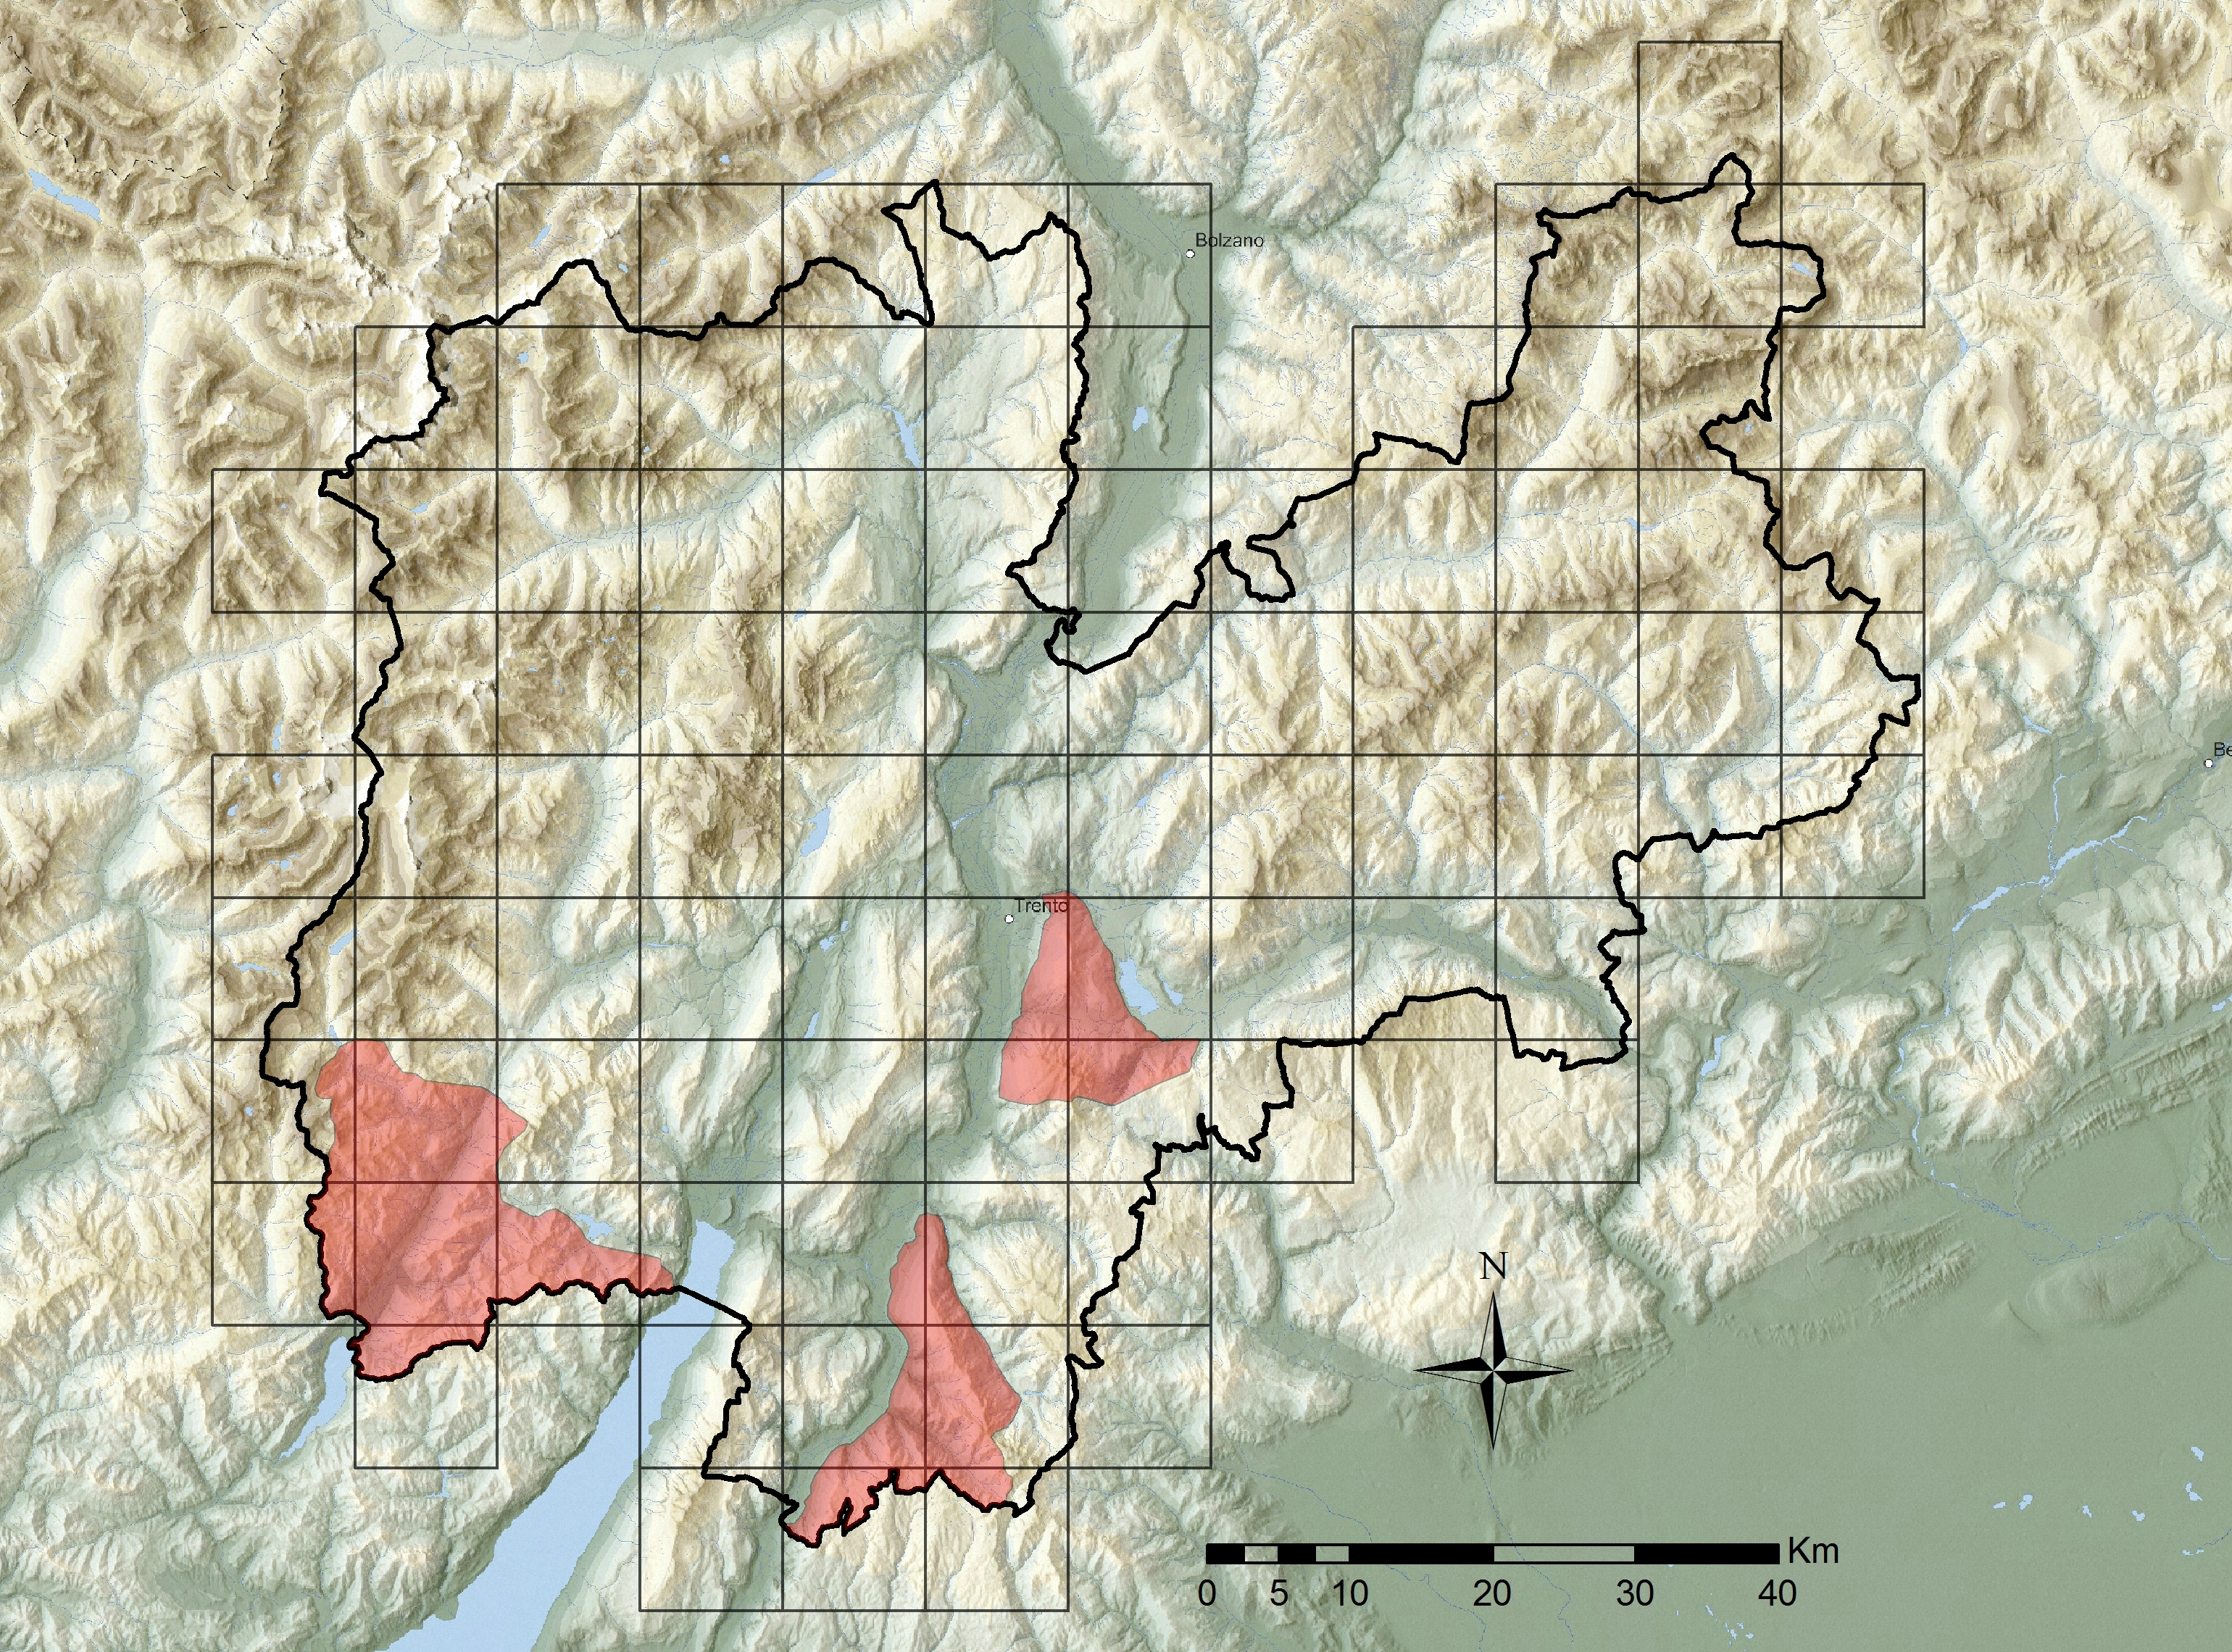
\includegraphics[width=.8\paperwidth]{06_Artiodattili/01_CINGHIALE/Sus_scrofa.jpg}
	\caption*{\tikzcircle[red,fill=red]{3pt} areale stimato}
\end{figure*}

\section{Preferenze ambientali}L{\textquoteright}habitat del cinghiale
si estende dalle aree intensamente coltivate e antropizzate della
pianura agli orizzonti montani coperti di boschi decidui e misti. Gli
unici fattori limitanti per la specie sembrano essere la presenza di
inverni rigidi caratterizzati dal forte innevamento o
l{\textquoteright}eccessivo sfruttamento delle aree agricole che porta
alla scomparsa delle zone boscate, indispensabili alla specie come zone
di rifugio. L{\textquoteright}ambiente prediletto \`e costituito da
boschi di querce alternati a cespuglieti e prati-pascoli con
sufficiente presenza di acqua. 

In Trentino, nelle zone di presenza, la specie \`e segnalata dalle zone
agricole di fondovalle fino a quote superiori ai 2000 metri.
Principalmente frequenta le aree di media e bassa montagna
caratterizzate da boschi di latifoglie. 

\section{Popolazione} Le prime segnalazioni della specie in provincia di
Trento risalgono al 1985 e interessano le aree del bacino del fiume
Chiese. L{\textquoteright}origine della diffusione di questi animali
\`e da ricondursi all{\textquoteright}immissione illegale, da parte dei
cacciatori locali, di due soggetti adulti e tre subadulti provenienti
da un{\textquoteright}azienda faunistico-venatoria della provincia di
Pisa.

\begin{Figure}
	\centering
	\includegraphics[width=.95\columnwidth]{./graph/R/SCRIPT/GRAPHS/Sus_scrofa_plot.pdf}
\end{Figure}
\captionof*{Figure}{Distribuzione altitudinale del cinghiale in Trentino}

Nonostante fosse stato sconsigliato al mondo venatorio di
procedere con simili attivit\`a, dato l{\textquoteright}elevato impatto
del cinghiale su numerose componenti dell{\textquoteright}ecosistema,
tra il 1990 e il 1991 analoghe segnalazioni provengono dalla Val
Rendena e dalla Val di Cembra. Immissioni di questo tipo sono avvenute,
fino almeno al 2007, in Valsugana, Val di Cembra e nelle Giudicarie. Di
dubbia provenienza sono i soggetti avvistati (dei quali alcuni
abbattuti) in Val di Sole e Destra Val di Non tra il 2012 e il 2014. 

Attualmente, in provincia di Trento \`e stimata una popolazione di circa
200-300 capi distribuiti principalmente in tre colonie: la prima in Val
del Chiese tra i confini con la provincia di Brescia e il corso del
fiume Chiese con circa 60-70 capi, la seconda tra Avio, Ala, Rovereto e
Vallarsa con circa 100-150 capi, mentre la terza, compresa tra la
Vigolana e la Marzola, consta di circa 60-70 capi. Il nucleo della
Valle di Ledro \`e di difficile quantificazione data
l{\textquoteright}ancora ridotta stabilit\`a dei contingenti sul
territorio trentino. 


\section{Notizie storiche} Il cronista del Concilio di Trento
Michel{\textquoteright}Angelo Mariani nel XVII secolo ricordava che
{\guillemotleft}ne{\textquoteright} M\"oti, Valli e luoghi pi\`u remoti
non mancano Daini, Camozzi, e Cervi; come ne meno Lupi, Orsi, e
tal{\textquoteright}hor Cignali\textit{{\guillemotright}}. Anche le
cronache di caccia del vicino Alto Adige annoveravano questa pregiata
specie di selvaggina come particolarmente frequente nei boschi di
querce e nelle paludi della Val d{\textquoteright}Adige. I danni che
questi animali procuravano alle campagne erano per\`o
tutt{\textquoteright}altro che limitati. Una precisa testimonianza in
questo senso, che riguarda il territorio trentino e pi\`u precisamente
alla Valsugana (Castelli 1941), \`e fornita da una missiva di Leopoldo
I (1640-1705) datata 27 aprile 1668, con la quale
l{\textquoteright}imperatore accoglieva le proteste del barone Giovanni
Andrea Giovanelli della Signoria di Telvana e dei suoi sudditi,
permettendo la caccia ai cervi e ai cinghiali, al fine di arginare i
danni che questi animali provocavano ai coltivi. Lo stesso imperatore
Leopoldo I qualche anno addietro, nel 1666, aveva addirittura fatto
emanare un apposito decreto allo scopo di eradicare la specie dal
Tirolo. L{\textquoteright}incremento della caccia fu tale che pochi
decenni pi\`u tardi, nel 1700, venne abbattuto presso Caldaro
l{\textquoteright}ultimo esemplare di cinghiale altoatesino, con la
conseguente estinzione locale della specie (Castelli 1940). 

Un atto della cancelleria vescovile datato 15 ottobre 1672 (Castelli
1941), per\`o, vietava in tutto il territorio del Principato di Trento
cacciare o acquistare varie specie di selvaggina, tra cui anche
{\textquotedblleft}porchi{\textquotedblright} e
{\textquotedblleft}cignali{\textquotedblright},
{\guillemotleft}constatato nel principato la penuria e scarsezza di
selvatici tanto volatili che quadrupedi (causa
l{\textquoteright}indiscreta e continua estradazione in alieni paesi)
onde provvedere che la citt\`a di Trento e territorio tutto non
scarseggi di quelle provvigioni che sono prodotte dalla naturale
fertilit\`a della propria patria{\guillemotright}. 

Una relazione, infine, del Tribunale circolare di Rovereto del 15 maggio
1807 (Castelli, 1941) accennava all{\textquoteright}assenza nel
territorio di propria pertinenza di cervi e cinghiali. La citazione di
quest{\textquoteright}ultima specie nel documento citato apparirebbe un
po{\textquoteright} strana se la scomparsa della stessa fosse avvenuta
pi\`u di un secolo prima. \`E quindi possibile che
l{\textquoteright}estinzione del cinghiale in Vallagarina abbia avuto
luogo nel XVIII secolo inoltrato.

Secondo Gregori (2002) il cinghiale era presente in Trentino fino al
XVIII secolo nella fascia dei querceti termofili della Valle
dell{\textquoteright}Adige e della Valsugana, nonch\'e in altre valli
meridionali della provincia. Massei e Toso (1993) riferiscono la
scomparsa della specie dal territorio provinciale al XVII secolo a
causa di un andamento climatico sfavorevole caratterizzato da periodi
molto freddi e umidi, caccia senza limitazioni, patologie quali ad
esempio la peste suina e riduzione dell{\textquoteright}habitat per
espansione delle coltivazioni a scapito dei querceti pedemontani e
delle residue formazioni planiziarie.


\section{Conservazione}  In questi ultimi anni il cinghiale ha assunto
un{\textquoteright}importanza venatoria progressivamente crescente con
notevoli conseguenze dirette e indirette, sia nei confronti della fauna
sia nella sua gestione. Se da un lato il mondo venatorio tende a
massimizzare le presenze operando con immissioni spesso abusive e
fortemente discutibili dal punto di vista tecnico e biologico,
dall{\textquoteright}altro si contrappone la necessit\`a di controllare
la densit\`a delle popolazioni che causano forti impatti sulle
attivit\`a agricole e su altri elementi della zoocenosi. 

Le immissioni venatorie sono iniziate con animali importati
dall{\textquoteright}estero, per poi proseguire con soggetti prodotti
in cattivit\`a in allevamenti nazionali, spesso sorvolando sui principi
della pianificazione faunistica e sulla profilassi sanitaria.
Nonostante le problematiche siano ormai note, persistono immissioni
pi\`u o meno abusive di questa specie, che compare progressivamente in
alcune aree dell{\textquoteright}arco alpino dove
l{\textquoteright}immigrazione spontanea da territori limitrofi sembra
da escludersi. 

La natura impattante del cinghiale si esercita in numerosi contesti. Nei
territori maggiormente interessati dalle produzioni agricole
l{\textquoteright}impatto del cinghiale su numerose essenze \`e dovuto
principalmente alle attivit\`a di scavo, tanto da richiedere fino
all{\textquoteright}80\% dei fondi a disposizione delle amministrazioni
provinciali per far fronte ai danni provocati dalla specie. La presenza
del cinghiale pu\`o avere impatti negativi su numerose altre specie
quali ad esempio i Cervidi e, fra l{\textquoteright}avifauna
nidificante, i Galliformi per predazione delle uova. Le immissioni
inoltre aumentano il rischio di diffusione di alcune malattie, quali la
tubercolosi e la peste suina, non solo nel cinghiale ma anche tra i
maiali domestici allevati.

La gestione di questa specie va spesso ben oltre le sole esigenze
ecologiche e deve affrontare problematiche culturali, sociali e
politiche che lasciano purtroppo poco spazio a una corretta
pianificazione faunistica.

Il Piano Faunistico Provinciale (PAT 2010) indica il divieto di
immettere in natura questa specie e impone l{\textquoteright}immediata
eradicazione di qualunque nuovo nucleo insediatosi sul territorio. Per
i nuclei gi\`a presenti sono invece previsti prelievi volti da un lato
a contenere i danni alle varie attivit\`a antropiche e
dall{\textquoteright}altro la salvaguardia degli habitat. La specie
attualmente non \`e cacciata ma sottoposta a piani di controllo nella
cui attuazione l{\textquoteright}amministrazione pubblica si avvale di
cacciatori espressamente formati e abilitati. 

\medskip
\medskip

{\raggedleft\itshape
Lucio Luchesa
}
\end{multicols}
\input{06_Artiodattili/02_CERVO/CERVO.tex}
\input{06_Artiodattili/03_CAPRIOLO/CAPRIOLO.tex}
\input{06_Artiodattili/04_MUFLONE/MUFLONE.tex}
\input{06_Artiodattili/05_STAMBECCO/STAMBECCO.tex}
\input{06_Artiodattili/06_CAMOSCIO/CAMOSCIO.tex}
\newpage
\input{06_Artiodattili/BIBLIOGRAFIA.tex}


%\part{Ordine Lagomorfi}
%\newpagecolor{white}\afterpage{\restorepagecolor}
%\pagestyle{empty}
%\input{03_Lagomorfi/01_LEPRE_COMUNE/LEPRE_COMUNE.tex}
%\input{03_Lagomorfi/02_LEPRE_BIANCA/LEPRE_BIANCA.tex}
%\input{03_Lagomorfi/03_CONIGLIO_SELVATICO/CONIGLIO_SELVATICO.tex}

%\part{Ordine Roditori}
%\newpagecolor{white}\afterpage{\restorepagecolor}
%\pagestyle{empty}
%\input{04_Roditori/RODITORI_intro.tex}
%\input{04_Roditori/03_GHIRO/GHIRO.tex}
%\input{04_Roditori/04_MOSCARDINO/MOSCARDINO.tex}
%\input{04_Roditori/05_QUERCINO/QUERCINO.tex}
%\input{04_Roditori/06_DRIOMIO/DRIOMIO.tex}
%\input{04_Roditori/07_ARVICOLA_DELLE_NEVI/ARVICOLA_DELLE_NEVI.tex}
%\input{04_Roditori/08_ARVICOLA_AGRESTE/ARVICOLA_AGRESTE.tex}
%\input{04_Roditori/09_ARVICOLA_CAMPESTRE/ARVICOLA_CAMPESTRE.tex}
%\input{04_Roditori/10_ARVICOLA_DEL_LIECHTENSTEIN/ARVICOLA_DEL_LIECHTENSTEIN.tex}
%\input{04_Roditori/11_ARVICOLA_DI_FATIO/ARVICOLA_DI_FATIO.tex}
%\input{04_Roditori/12_ARVICOLA_SOTTERRANEA/ARVICOLA_SOTTERRANEA.tex}
%\input{04_Roditori/13_ARVICOLA_ROSSASTRA/ARVICOLA_ROSSASTRA.tex}
%\input{04_Roditori/15_TOPO_SELVATICO_A_COLLO_GIALLO/TOPO_SELVATICO_A_COLLO_GIALLO.tex}
%\input{04_Roditori/16_TOPO_SELVATICO/TOPO_SELVATICO.tex}
%\input{04_Roditori/18_TOPOLINO_DOMESTICO/TOPOLINO_DOMESTICO.tex}
%\input{04_Roditori/19_RATTO_DELLE_CHIAVICHE/RATTO_DELLE_CHIAVICHE.tex}
%\input{04_Roditori/20_RATTO_NERO/RATTO_NERO.tex}

%\part{Ordine Carnivori}
%\newpagecolor{white}\afterpage{\restorepagecolor}
%\pagestyle{empty}
%\input{05_Carnivori/01_SCIACALLO_DORATO/SCIACALLO_DORATO.tex}
%\input{05_Carnivori/03_VOLPE/VOLPE.tex}
%\input{05_Carnivori/04_ORSO_BRUNO/ORSO_BRUNO.tex}
%\input{05_Carnivori/05_FAINA/FAINA.tex}
%\input{05_Carnivori/06_MARTORA/MARTORA.tex}
%\input{05_Carnivori/07_ERMELLINO/ERMELLINO.tex}
%\input{05_Carnivori/08_DONNOLA/DONNOLA.tex}
%\input{05_Carnivori/09_PUZZOLA/PUZZOLA.tex}
%\input{05_Carnivori/10_TASSO/TASSO.tex}
%\input{05_Carnivori/13_LINCE/LINCE.tex}

%\part{Ordine Artiodattili}
%\newpagecolor{white}\afterpage{\restorepagecolor}
%\pagestyle{empty}
%\input{06_Artiodattili/ARTIODATTILI_intro.tex}
%\pagestyle{ATLASpage}

\afterchapterparagraph{
	\vspace{-10pt}
	\noindent\color{MUSE}\rule{27cm}{1pt}
	\index{Lucio Luchesa}
}
\chapter[Cinghiale - \textit{Sus scrofa} (Linnaeus, 1758)]{\textbf{Cinghiale}  \\[2pt] {\LARGE\textit{Sus scrofa} (Linnaeus, 1758)}}
\vspace{5pt}\\

\begin{center}
	\includegraphics[height=.3\paperheight]{06_Artiodattili/01_CINGHIALE/Sus_scrofa_MG.jpg}
\end{center}
{\hspace*{\fill}\footnotesize\itshape Paolo Paolucci}
\begin{multicols}{2}
\section{Sottospecie}Fattori di origine principalmente antropica
consentono di definire dubbia la sistematica del cinghiale. La
situazione creatasi a causa delle ripetute ibridazioni del suide con i
conspecifici domestici, \`e stata ulteriormente complicata dai numerosi
fenomeni di incrocio con forme evolutesi in aree geografiche
differenti, utilizzate dall{\textquoteright}uomo per molteplici
attivit\`a di immissione.

Le attuali incertezze sul reale significato delle 16 sottospecie di
cinghiale formalmente riconosciute (Mitchell \textit{et al.} 1999),
fanno s\`i che ci si limiti ad individuare quattro informali
raggruppamenti geografici regionali, ai quali le sottospecie fanno
riferimento dal punto di vista morfologico: razze occidentali, indiane,
orientali e indonesiane. 

Per quanto riguarda il territorio italiano, la forma autoctona che
abitava, un tempo, la parte settentrionale della penisola \`e scomparsa
prima che potesse essere effettuata una sua caratterizzazione
sistematica e tassonomica, mentre carenti risultano essere le
informazioni sulle origini della popolazione sarda, rappresentata da
\textit{Sus scrofa meridionalis} e della popolazione maremmana,
identificata in \textit{S. s. majori}. Indagini genetiche e
morfometriche sottolineano come non vi sia differenza tra la
popolazione maremmana e quella presente nella restante parte della
penisola (\textit{S. s. scrofa}), mentre la sottospecie sarda,
differenziata sia geneticamente che morfologicamente, pare essersi
originata da popolazioni domestiche anticamente rinselvatichite.


\section{Distribuzione} La grande adattabilit\`a alle diverse condizioni
ecologiche che caratterizza il cinghiale, \`e
l{\textquoteright}elemento chiave per comprendere il considerevole
ampliamento del suo areale avvenuto in tutta Europa negli ultimi
decenni. Spagna, Francia, Finlandia, Russia europea, Repubblica Ceca e
Slovacchia, sono solo alcune delle nazioni interessate dalla presenza
di questa specie, che con una superficie che si estende per circa
190.000 km\textsuperscript{2}, fa del cinghiale
l{\textquoteright}ungulato pi\`u diffuso in Italia, sia in termini
distributivi che di consistenza. La specie \`e diffusa senza soluzione
di continuit\`a dalla Liguria, attraverso gli Appennini, sino alla
Calabria e in tutta la Sardegna, a eccezione delle province di Brindisi
e Lecce. La Sicilia \`e stata invece recente oggetto di immissioni. Per
quanto riguarda il territorio alpino e prealpino, la presenza della
specie \`e continua in tutta l{\textquoteright}area occidentale
(Piemonte e Valle d{\textquoteright}Aosta) ed \`e in particolare
espansione in quella orientale (Friuli Venezia Giulia). Nella parte
centrale delle Alpi si sta assistendo a una rapida espansione
dell{\textquoteright}areale distributivo, tanto da rendere
ipotizzabile, a breve, la saldatura delle popolazioni della parte
orientale e di quella occidentale delle Alpi. La specie \`e stabilmente
presente, con densit\`a ancora relativamente basse, nella zona
collinare e montana della provincia di Verona (Lessinia), nel Trentino
meridionale, sia in sinistra che in destra orografica del fiume Adige
(Vallagarina, Valsugana, Valle di Ledro, bassa Valle del Chiese), nella
zona montana della provincia di Vicenza e di Treviso e nel Pordenonese.
Anche nella zona delle Alpi e Prealpi della Lombardia la specie ha
oramai attestato la presenza su un fronte che dall{\textquoteright}Alto
Garda bresciano prosegue fino ai confini con il Piemonte. 


\section{Distribuzione in Trentino} In provincia di Trento il cinghiale
occupa stabilmente la sinistra orografica dell{\textquoteright}Adige,
dal Leno di Vallarsa fino ai confini con le province di Verona e
Vicenza. L{\textquoteright}insediamento del nucleo che occupa
quest{\textquoteright}area \`e stato determinato da immigrazione
naturale di soggetti dal veronese. Un secondo nucleo, riproduttivo
almeno dal 2007, \`e localizzato sul massiccio della Vigolana, sia sul
versante meridionale che su quello settentrionale e sulla Marzola.
Singoli soggetti in espansione sono segnalati nel territorio -- in
sinistra orografica del fiume Adige -- che separa queste due aree. 

La parte di territorio provinciale che per prima \`e stata interessata
dalla presenza del suide \`e la bassa Valle del Chiese nella quale il
cinghiale risulta presente principalmente nella porzione in destra
orografica del fiume Chiese. La specie in quest{\textquoteright}area
\`e stata introdotta illegalmente nella prima met\`a degli anni Ottanta
dello scorso secolo. La parte meridionale della Valle di Ledro \`e
sempre pi\`u interessata dalla presenza della specie a causa dei
fenomeni di immigrazione dal confinante Alto Garda bresciano. 

Recentemente il cinghiale \`e segnalato anche sul Monte Baldo, sia sul
versante orientale che su quello occidentale:
l{\textquoteright}espansione verso la parte settentrionale del
complesso montuoso, partita dal territorio veronese -- e in forma
ridotta per attraversamento del fiume Adige nella zona compresa tra gli
abitati di Serravalle e Pilcante di Ala -- ha portato
nell{\textquoteright}ultimo biennio ad una stabile presenza, seppur di
solo qualche soggetto, nel comune di Nago-Torbole.

Nel rimanente territorio provinciale occasionalmente sono stati
segnalati singoli soggetti erratici. 

\begin{figure*}
	\centering
	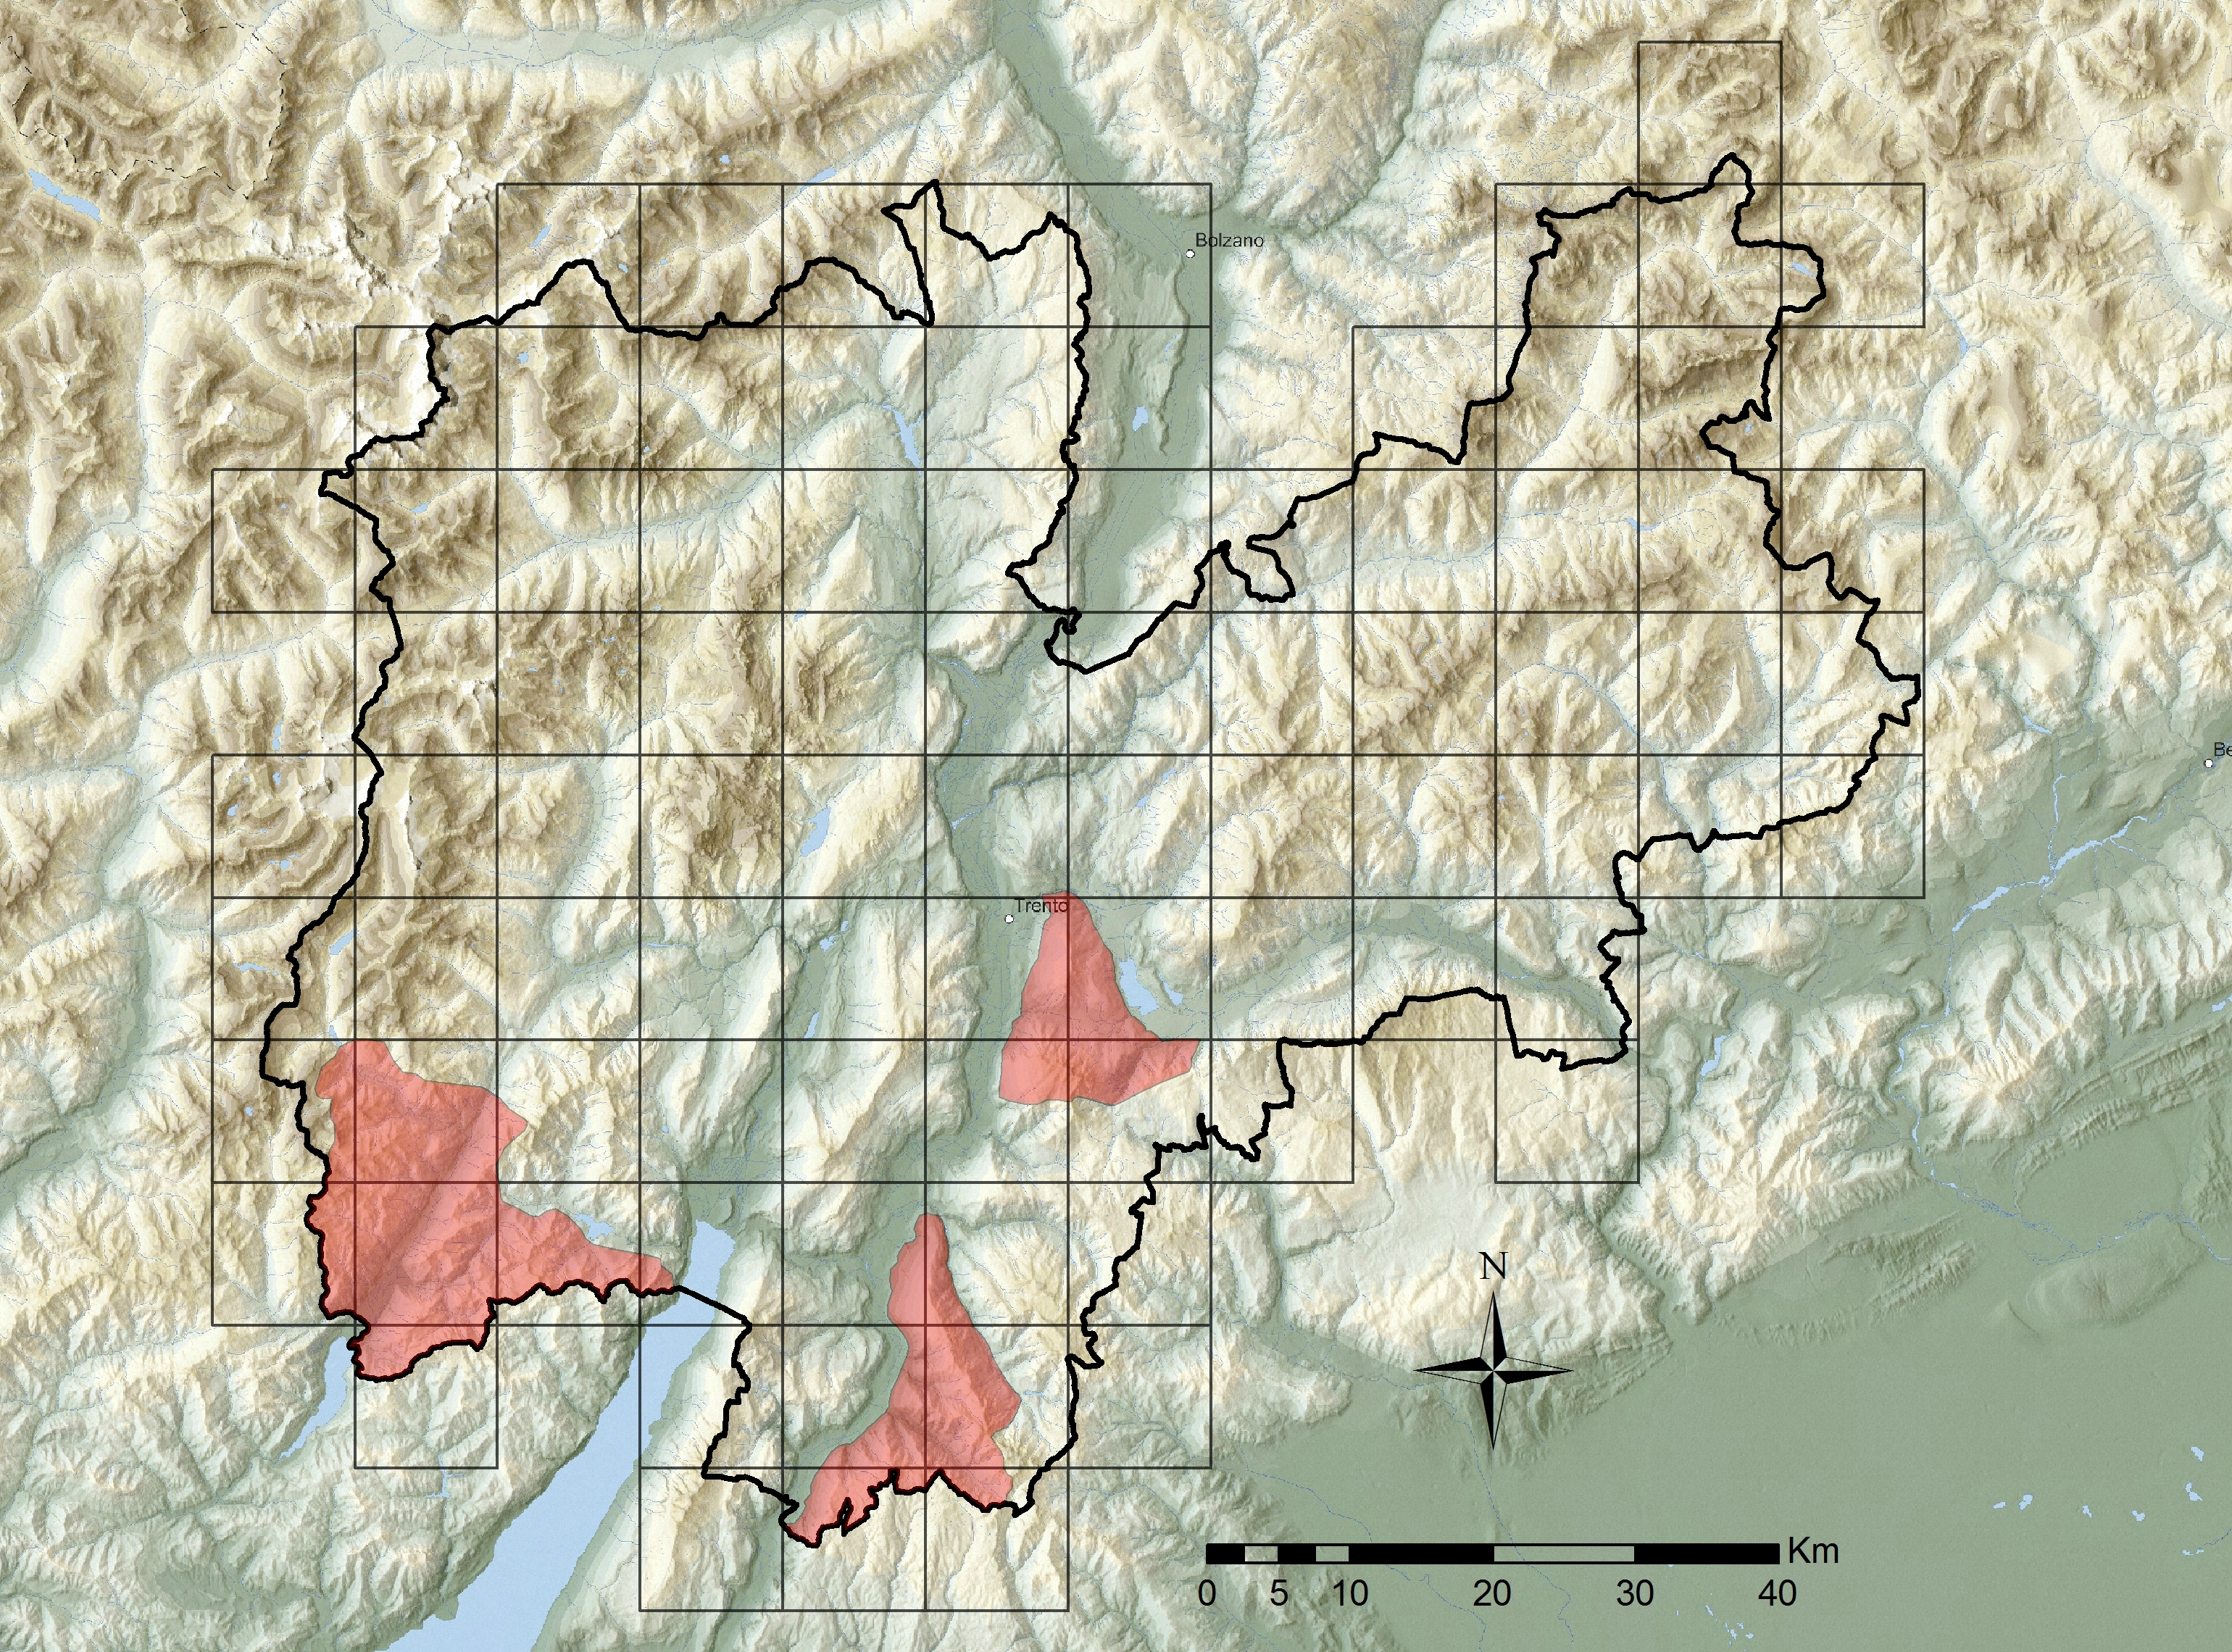
\includegraphics[width=.8\paperwidth]{06_Artiodattili/01_CINGHIALE/Sus_scrofa.jpg}
	\caption*{\tikzcircle[red,fill=red]{3pt} areale stimato}
\end{figure*}

\section{Preferenze ambientali}L{\textquoteright}habitat del cinghiale
si estende dalle aree intensamente coltivate e antropizzate della
pianura agli orizzonti montani coperti di boschi decidui e misti. Gli
unici fattori limitanti per la specie sembrano essere la presenza di
inverni rigidi caratterizzati dal forte innevamento o
l{\textquoteright}eccessivo sfruttamento delle aree agricole che porta
alla scomparsa delle zone boscate, indispensabili alla specie come zone
di rifugio. L{\textquoteright}ambiente prediletto \`e costituito da
boschi di querce alternati a cespuglieti e prati-pascoli con
sufficiente presenza di acqua. 

In Trentino, nelle zone di presenza, la specie \`e segnalata dalle zone
agricole di fondovalle fino a quote superiori ai 2000 metri.
Principalmente frequenta le aree di media e bassa montagna
caratterizzate da boschi di latifoglie. 

\section{Popolazione} Le prime segnalazioni della specie in provincia di
Trento risalgono al 1985 e interessano le aree del bacino del fiume
Chiese. L{\textquoteright}origine della diffusione di questi animali
\`e da ricondursi all{\textquoteright}immissione illegale, da parte dei
cacciatori locali, di due soggetti adulti e tre subadulti provenienti
da un{\textquoteright}azienda faunistico-venatoria della provincia di
Pisa.

\begin{Figure}
	\centering
	\includegraphics[width=.95\columnwidth]{./graph/R/SCRIPT/GRAPHS/Sus_scrofa_plot.pdf}
\end{Figure}
\captionof*{Figure}{Distribuzione altitudinale del cinghiale in Trentino}

Nonostante fosse stato sconsigliato al mondo venatorio di
procedere con simili attivit\`a, dato l{\textquoteright}elevato impatto
del cinghiale su numerose componenti dell{\textquoteright}ecosistema,
tra il 1990 e il 1991 analoghe segnalazioni provengono dalla Val
Rendena e dalla Val di Cembra. Immissioni di questo tipo sono avvenute,
fino almeno al 2007, in Valsugana, Val di Cembra e nelle Giudicarie. Di
dubbia provenienza sono i soggetti avvistati (dei quali alcuni
abbattuti) in Val di Sole e Destra Val di Non tra il 2012 e il 2014. 

Attualmente, in provincia di Trento \`e stimata una popolazione di circa
200-300 capi distribuiti principalmente in tre colonie: la prima in Val
del Chiese tra i confini con la provincia di Brescia e il corso del
fiume Chiese con circa 60-70 capi, la seconda tra Avio, Ala, Rovereto e
Vallarsa con circa 100-150 capi, mentre la terza, compresa tra la
Vigolana e la Marzola, consta di circa 60-70 capi. Il nucleo della
Valle di Ledro \`e di difficile quantificazione data
l{\textquoteright}ancora ridotta stabilit\`a dei contingenti sul
territorio trentino. 


\section{Notizie storiche} Il cronista del Concilio di Trento
Michel{\textquoteright}Angelo Mariani nel XVII secolo ricordava che
{\guillemotleft}ne{\textquoteright} M\"oti, Valli e luoghi pi\`u remoti
non mancano Daini, Camozzi, e Cervi; come ne meno Lupi, Orsi, e
tal{\textquoteright}hor Cignali\textit{{\guillemotright}}. Anche le
cronache di caccia del vicino Alto Adige annoveravano questa pregiata
specie di selvaggina come particolarmente frequente nei boschi di
querce e nelle paludi della Val d{\textquoteright}Adige. I danni che
questi animali procuravano alle campagne erano per\`o
tutt{\textquoteright}altro che limitati. Una precisa testimonianza in
questo senso, che riguarda il territorio trentino e pi\`u precisamente
alla Valsugana (Castelli 1941), \`e fornita da una missiva di Leopoldo
I (1640-1705) datata 27 aprile 1668, con la quale
l{\textquoteright}imperatore accoglieva le proteste del barone Giovanni
Andrea Giovanelli della Signoria di Telvana e dei suoi sudditi,
permettendo la caccia ai cervi e ai cinghiali, al fine di arginare i
danni che questi animali provocavano ai coltivi. Lo stesso imperatore
Leopoldo I qualche anno addietro, nel 1666, aveva addirittura fatto
emanare un apposito decreto allo scopo di eradicare la specie dal
Tirolo. L{\textquoteright}incremento della caccia fu tale che pochi
decenni pi\`u tardi, nel 1700, venne abbattuto presso Caldaro
l{\textquoteright}ultimo esemplare di cinghiale altoatesino, con la
conseguente estinzione locale della specie (Castelli 1940). 

Un atto della cancelleria vescovile datato 15 ottobre 1672 (Castelli
1941), per\`o, vietava in tutto il territorio del Principato di Trento
cacciare o acquistare varie specie di selvaggina, tra cui anche
{\textquotedblleft}porchi{\textquotedblright} e
{\textquotedblleft}cignali{\textquotedblright},
{\guillemotleft}constatato nel principato la penuria e scarsezza di
selvatici tanto volatili che quadrupedi (causa
l{\textquoteright}indiscreta e continua estradazione in alieni paesi)
onde provvedere che la citt\`a di Trento e territorio tutto non
scarseggi di quelle provvigioni che sono prodotte dalla naturale
fertilit\`a della propria patria{\guillemotright}. 

Una relazione, infine, del Tribunale circolare di Rovereto del 15 maggio
1807 (Castelli, 1941) accennava all{\textquoteright}assenza nel
territorio di propria pertinenza di cervi e cinghiali. La citazione di
quest{\textquoteright}ultima specie nel documento citato apparirebbe un
po{\textquoteright} strana se la scomparsa della stessa fosse avvenuta
pi\`u di un secolo prima. \`E quindi possibile che
l{\textquoteright}estinzione del cinghiale in Vallagarina abbia avuto
luogo nel XVIII secolo inoltrato.

Secondo Gregori (2002) il cinghiale era presente in Trentino fino al
XVIII secolo nella fascia dei querceti termofili della Valle
dell{\textquoteright}Adige e della Valsugana, nonch\'e in altre valli
meridionali della provincia. Massei e Toso (1993) riferiscono la
scomparsa della specie dal territorio provinciale al XVII secolo a
causa di un andamento climatico sfavorevole caratterizzato da periodi
molto freddi e umidi, caccia senza limitazioni, patologie quali ad
esempio la peste suina e riduzione dell{\textquoteright}habitat per
espansione delle coltivazioni a scapito dei querceti pedemontani e
delle residue formazioni planiziarie.


\section{Conservazione}  In questi ultimi anni il cinghiale ha assunto
un{\textquoteright}importanza venatoria progressivamente crescente con
notevoli conseguenze dirette e indirette, sia nei confronti della fauna
sia nella sua gestione. Se da un lato il mondo venatorio tende a
massimizzare le presenze operando con immissioni spesso abusive e
fortemente discutibili dal punto di vista tecnico e biologico,
dall{\textquoteright}altro si contrappone la necessit\`a di controllare
la densit\`a delle popolazioni che causano forti impatti sulle
attivit\`a agricole e su altri elementi della zoocenosi. 

Le immissioni venatorie sono iniziate con animali importati
dall{\textquoteright}estero, per poi proseguire con soggetti prodotti
in cattivit\`a in allevamenti nazionali, spesso sorvolando sui principi
della pianificazione faunistica e sulla profilassi sanitaria.
Nonostante le problematiche siano ormai note, persistono immissioni
pi\`u o meno abusive di questa specie, che compare progressivamente in
alcune aree dell{\textquoteright}arco alpino dove
l{\textquoteright}immigrazione spontanea da territori limitrofi sembra
da escludersi. 

La natura impattante del cinghiale si esercita in numerosi contesti. Nei
territori maggiormente interessati dalle produzioni agricole
l{\textquoteright}impatto del cinghiale su numerose essenze \`e dovuto
principalmente alle attivit\`a di scavo, tanto da richiedere fino
all{\textquoteright}80\% dei fondi a disposizione delle amministrazioni
provinciali per far fronte ai danni provocati dalla specie. La presenza
del cinghiale pu\`o avere impatti negativi su numerose altre specie
quali ad esempio i Cervidi e, fra l{\textquoteright}avifauna
nidificante, i Galliformi per predazione delle uova. Le immissioni
inoltre aumentano il rischio di diffusione di alcune malattie, quali la
tubercolosi e la peste suina, non solo nel cinghiale ma anche tra i
maiali domestici allevati.

La gestione di questa specie va spesso ben oltre le sole esigenze
ecologiche e deve affrontare problematiche culturali, sociali e
politiche che lasciano purtroppo poco spazio a una corretta
pianificazione faunistica.

Il Piano Faunistico Provinciale (PAT 2010) indica il divieto di
immettere in natura questa specie e impone l{\textquoteright}immediata
eradicazione di qualunque nuovo nucleo insediatosi sul territorio. Per
i nuclei gi\`a presenti sono invece previsti prelievi volti da un lato
a contenere i danni alle varie attivit\`a antropiche e
dall{\textquoteright}altro la salvaguardia degli habitat. La specie
attualmente non \`e cacciata ma sottoposta a piani di controllo nella
cui attuazione l{\textquoteright}amministrazione pubblica si avvale di
cacciatori espressamente formati e abilitati. 

\medskip
\medskip

{\raggedleft\itshape
Lucio Luchesa
}
\end{multicols}
%\input{06_Artiodattili/02_CERVO/CERVO.tex}
%\input{06_Artiodattili/03_CAPRIOLO/CAPRIOLO.tex}
%\input{06_Artiodattili/04_MUFLONE/MUFLONE.tex}
%\input{06_Artiodattili/05_STAMBECCO/STAMBECCO.tex}
%\input{06_Artiodattili/06_CAMOSCIO/CAMOSCIO.tex}
%\newpage
%\input{06_Artiodattili/BIBLIOGRAFIA.tex}

\end{document}
